% !TEX root = ../AiiDA_tutorial.tex
\section{Queries in AiiDA - Optional examples and exercises}


\subsection*{Optional exercises on relationships (Task 3)}
\textbf{Hint for the exercises:}
\begin{itemize}
\item You can have projections on properties of more than one entity in your query. You just have to add the \emph{project} key (specifying the list of properties that you want to project) along with the corresponding entity when you append it.
\end{itemize}

\begin{tcolorbox}
\textbf{Exercises:}\\~\\
Try to write the following queries:
\begin{itemize}
	\item Find all descendants of a StructureData with a certain uuid. Print both the StructureData and the descendant.
	\item Find all the FolderData created by a specific user.
\end{itemize}
\end{tcolorbox}

\subsection*{Optional exercises on attributes and extras (Task 4)}
\textbf{Hint for the exercises:}
\begin{itemize}
\item You can easily order or limit the number of the results by using the \emph{order\_by()} and \emph{limit()} methods of the QueryBuilder. For example, we can order all our job calculation by their \textit{id} and limit the result to the first 10 as follows:
\begin{pythoncommand}
qb = QueryBuilder()
qb.append(JobCalculation, tag='calc')
qb.order_by({'calc':'id'})
qb.limit(10)
qb.all()
\end{pythoncommand}
\end{itemize}

\begin{tcolorbox}
\textbf{Exercises:}
\begin{itemize}
    \item Write a code snippet that informs you how many pseudopotentials you have for each element.
    \item Smearing contribution to the total energy for calculations:
    \begin{enumerate}
        \item Write a query that returns the smearing contribution to the energy stored in some instances of ParameterData.
        \item Extend the previous query to also get the input structures.
        \item Which structures have a smearing contribution to the energy smaller or equal to -0.02?
    \end{enumerate}
\end{itemize}
\end{tcolorbox}

\subsection*{Summarizing what we learned by now - An example}
At this point you should be able to do queries with projections, joins and filters. Moreover, you saw how to apply filters and projections even on attributes and extras. Let's discover the full power of the QueryBuilder with a complex graph query that allows you to project various properties from different nodes and apply different filters and joins.

Imagine that you would like to get the smearing energy for all the calculations that have finished and have a $\mathrm{Sn_{2}O_{3}}$ as input. Moreover, besides from the smearing energy, you would like to print the units of this energy and the formula of the structure that was given to the calculation.
The graphical representation of this query can be seen in Figure~\ref{fig:qb2} and the actual query follows:
\begin{figure}[!th]
\begin{center}
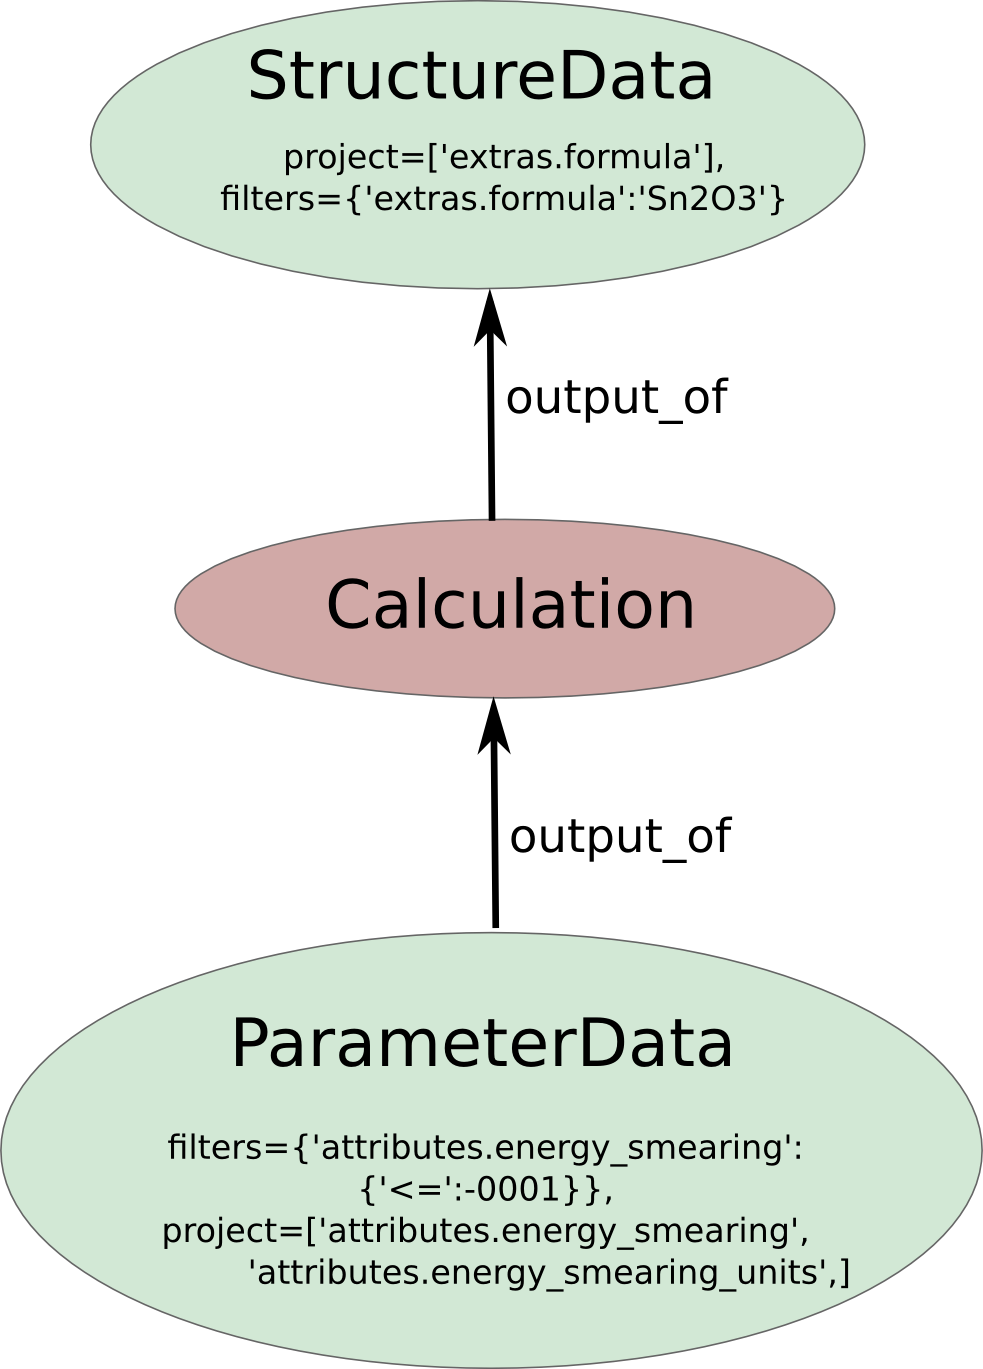
\includegraphics[width=7cm]{img/qb_example_2.png}
\end{center}
\caption{Complex graph query.}
\label{fig:qb2}
\end{figure}

\begin{pythoncommand}
qb = QueryBuilder()
qb.append(
        StructureData,
        project=["extras.formula"],
        filters={"extras.formula":"Sn2O3"},
        tag="structure"
    )
qb.append(
        Calculation,
        tag="calculation",
        output_of="structure"
    )
qb.append(
        ParameterData,
        tag="results",
        filters={"attributes.energy_smearing":{"<=":-0.0001}},
        project=[
            "attributes.energy_smearing",
            "attributes.energy_smearing_units",
        ],
        output_of="calculation"
)
qb.all()
\end{pythoncommand}

\section{\label{sec:convpressure}More complex logic in workflows: while loops and conditional statements}
In the previous sections, you have been introduced to WorkChains, and the reason for using them over ``standard'' workfunctions (i.e., functions decorated with \cmd{@wf}).

However, in the example of Sec.~\ref{sec:workchainsimple}, the \cmd{spec.outline} was quite simple, with a ``static'' sequence of two steps.
Most often, however, you need dynamic workflows, where you need to decide at runtime whether to continue to compute or not (e.g. in a convergence loop, where you need to stop if convergence has been achieved).
To support this scenario, the \cmd{spec.outline} can support logic: \emph{while} loops and \emph{if/elif/else} blocks.
The simplest way to explain it is to show an example:
\begin{pythoncommand}
from aiida.work.workchain import if_, while_

spec.outline(
    cls.s1,
    if_(cls.isA)(
        cls.s2
    ).elif_(cls.isB)(
        cls.s3
    ).else_(
        cls.s4
    ),
    cls.s5,
    while_(cls.condition)(
        cls.s6
    ),
)
\end{pythoncommand}
that would \emph{roughly} correspond, in a python syntax, to:
\begin{pythoncommand}
s1()
if isA():
    s2()
elif isB():
    s3()
else:
    s4()
s5()
while condition():
    s6()
\end{pythoncommand}
The only constraint is that condition functions (in the example above \cmd{isA}, \cmd{isB} and \cmd{condition}) must be class methods that returns \texttt{True} or \texttt{False} depending on whether the condition is met or not.

A suggestion on how to write new workchains: Use the outline to help you in designing the logic. First create the spec outline writing, almost if you were explaining it in words, what you expect the workflow to do. Then, define one by one the methods.
For example, we have prepared a simple workfunction to optimize the lattice parameter of silicon efficiently using a Newton's algorithm on the energy derivative, i.e. the pressure $p=-dE/dV$. You can find it the code at \texttt{tutorial\_scripts/pressure\_convergence.py}. 
The outline looks like this:
\begin{pythoncommand}
spec.outline(
    cls.init,
    cls.put_step0_in_ctx,
    cls.move_next_step,
    while_(cls.not_converged)(
        cls.move_next_step,
     ),
    cls.report
)
\end{pythoncommand}
This outline already roughly explains the algorithm: after an initialization (\cmd{init}) and putting the first step (number zero) in the ctx (\cmd{put\_step0\_in\_ctx}), a function to move to the next step is called (\cmd{move\_next\_step}). This is iterated while a given convergence criterion is not met (\cmd{not\_converged}). Finally, some reporting is done, including returning some output nodes (\cmd{report}).

If you are interested in the details of the algorithm, you can inspect the file. The main ideas are described here:
\begin{description}
\item[init] Generate a \texttt{pw.x} calculation for the input structure (with volume $V$), and one for a structure where the volume is $V+4\text{\AA}^3$ (just to get a closeby volume). Store the results in the context as \cmd{r0} and \cmd{r1}
\item[put\_step0\_in\_ctx] Store in the context $V$, $E(V)$ and $dE/dV$ for the first calculation \cmd{r0}
\item[move\_next\_step] This is the most important function. Calculate $V$, $E(V)$ and $dE/dV$ for \cmd{r1}. Also, estimate $d^2E/dV^2$ from the finite difference of the first derivative of \cmd{r0} and \cmd{r1} (helper functions to achieve this are provided).
Get the $a$, $b$ and $c$ coefficients of a parabolic fit $E=aV^2 + bV + c$ and estimated the expected minimum of the EOS function as the minimum of the fit $V_0=-b/2a$. Finally, replace \cmd{r0} with \cmd{r1} in the context (i.e., get rid of the oldest point) and launch a new pw calculation at volume $V_0$, that will be stored in the context replacing \cmd{r1}. In this way, at the next iteration \cmd{r0} and \cmd{r1} will contain the latest two simulations. Finally, at each step some relevant information (coefficients $a$, $b$ and $c$, volumes, energies, energy derivatives, ...) are stored in a list called \cmd{steps}. This whole list is stored in the context because it provides quantities to be preserved between different workfunction steps.
\item[not\_converged] Return \cmd{True} if convergence has not been achieved yet. Convergence is achieved if the difference in volume between the two latest simulations is smaller than a given threshold (\cmd{volume\_tolerance}).
\item[report] This is the final step. Mainly, we return the output nodes: \cmd{steps} with the list of results at each step, and \cmd{structure} with the final converged structure.
\end{description}

The results returned in \cmd{steps} can be used to represent the evolution of the minimisation algorithm. A possible way to visualize it is presented in Fig.~\ref{fig:convpressure}, obtained with an initial lattice constant of $a_{\text{lat}} = 5.2\text{\AA}$. 
%You can try to reproduce the same graph by running the WorkChain and then using the script \texttt{tutorial\_scripts/plot\_convergence\_pressure.py} to generate the same plot.

\begin{figure}[tb]
\centering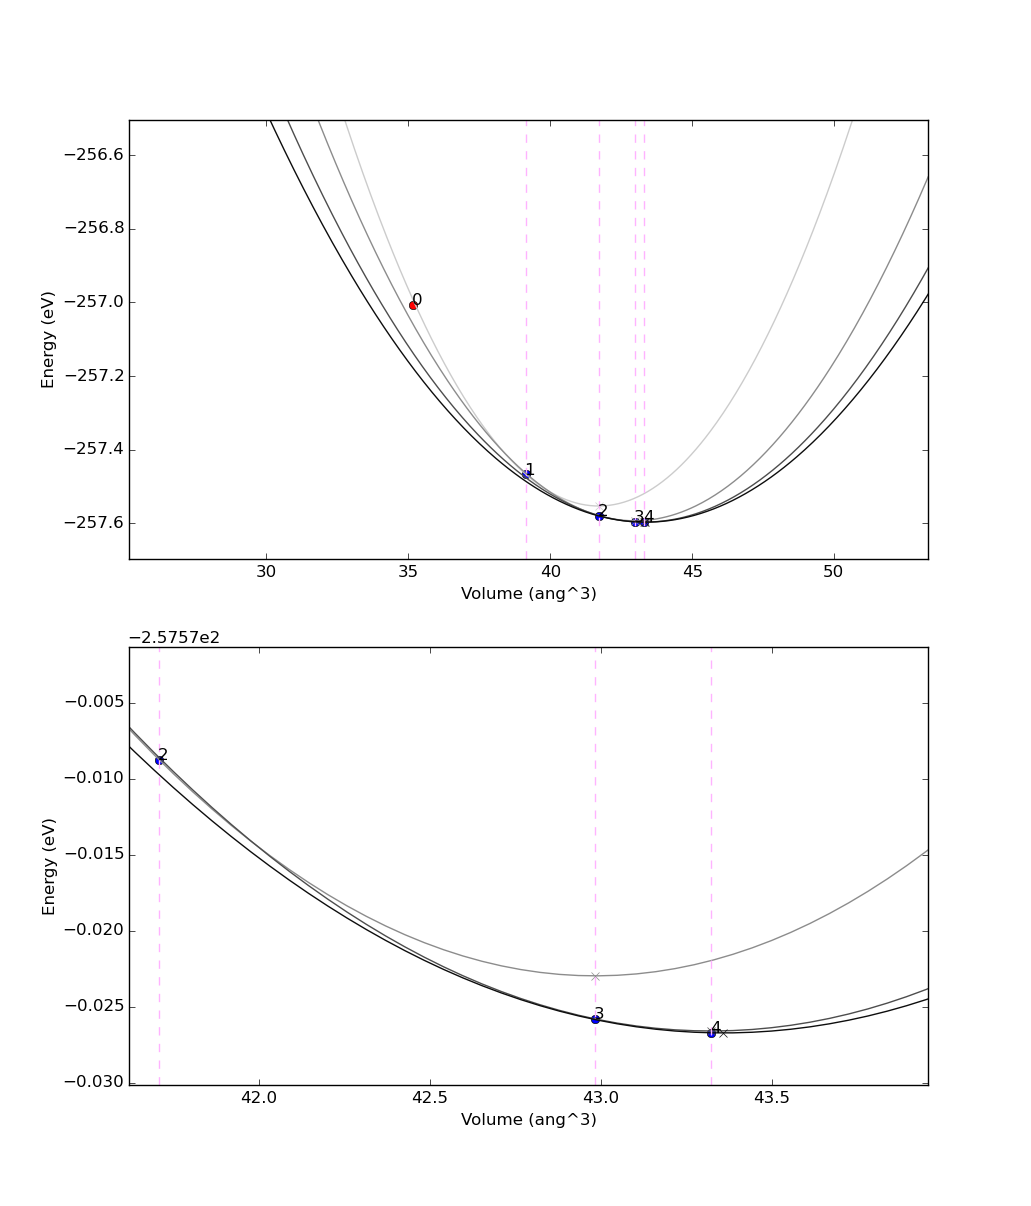
\includegraphics[width=0.6\linewidth]{img/convergence_pressure}
\caption{\label{fig:convpressure}Example of results of the convergence algorithm presented in Sec.~\ref{sec:convpressure}. The bottom plot is a zoom near the minimum. The dots represent the (volume,energy) points obtained from Quantum ESPRESSO, and the numbers indicate at which iteration they were obtained. The parabolas represent the parabolic fits used in the algorithm; the minimum of the parabola is represented with a small cross, in correspondence of the vertical lines, used as the volume for the following step.}
\end{figure} 


